%--------------------------------------------------------------------------------------------------
% OBSERVACAO:
% 
% -> Arquivos que você pode editar:
%    - artigo.tex
%    - artigo_bibliografia.bib
%
% -> Arquivo .TeX codificado em UTF8                                                             
% -> Bibliografia em arquivo .bib (arquivo_bibliografia.bib)                                      
% -> Arquivo de imagens em .jpg, .eps ou .pdf
% -> Para compilar o TeX, execute 'compila_TEX.bat' (terminal do windows)
% 
% versão 1.1 - 19/05/2016
% versão 1.0 - 18/08/2015
%--------------------------------------------------------------------------------------------------
\documentclass{classe_cn}                 % Modelo <nao edite o arquivo classe_cn.cls>
\usepackage[brazil]{babel}                % Acentos
\usepackage[utf8]{inputenc}               % Codificação UTF8 (atenção aqui!)
\usepackage{graphicx}                     % Figura
\usepackage{amssymb}                      % Simbolos matematicos
\usepackage{color}                        % Cores
\usepackage{amsfonts}                     % Fontes
\usepackage{amsmath}                      % Fontes
\usepackage[fixlanguage]{babelbib}        % Acentos
\usepackage[normalem]{ulem}               % OK
\usepackage[retainorgcmds]{IEEEtrantools} % Formulas padrão IEEE
\usepackage{omlmathbf}                    % Simbolos Matematicos
\usepackage{epstopdf}                     % Figuras .eps
\usepackage{setspace}                     % Espaçamento flexível
\usepackage{cmap}                         % Mapear caracteres especiais no PDF
\usepackage{textcomp}                     % Funções e outros símbolos matemáticos
\usepackage{verbatim}                     % Pacotes verbatim
\usepackage{wrapfig}
%\usepackage{picins}
\startlocaldefs
\endlocaldefs

%--------------------------------------------------------------------------------------------------
% Inicio do Documento
%--------------------------------------------------------------------------------------------------
\begin{document}
\begin{frontmatter}        % Não alterar
\begin{fmbox}              % Não alterar
\dochead{Gerência da Informação} % Não alterar

%--------------------------------------------------------------------------------------------------
% Titulo do seu Trabalho
%   - pequeno bug (nao funciona cedilha)
%   - editar manualmente o cedilha na classe_cn.cls, linha 1015.
%--------------------------------------------------------------------------------------------------
\title{O Modelo de Crowdfunding}

%------------------------------------------------
% Informações sobre o autor #1
% - Ivete Maria Dias de Sangalo
%------------------------------------------------
\author[
  addressref = {ricardo1},                 % Identifica o autor #1
  email      = {ricardo.maia@ccc.ufcg.edu.br} % email para contato
]
{
  \inits{RdAM}      % Letras iniciais do autor #1
  \fnm{Ricardo de A.}  % Nome do autor #1 (first and middle name)
  \snm{Maia}   % Ultimo nome do autor #1 (last name)
}
%------------------------------------------------
% Informações sobre o autor #2
% - James Alan Hetfield
%------------------------------------------------
\author[
  addressref = {danielle2},                      % Identifica o autor
  email      = {danielle.vieira@ccc.ufcg.edu.br} % email para contato
]
{
  \inits{DdLV}       % Letras iniciais do autor #2
  \fnm{Danielle de L.}  % Nome do autor #2 (first and middle name)
  \snm{Vieira}    % Ultimo nome do autor #2 (last name)
}
%------------------------------------------------
% Informações sobre o autor #3
% - Freddie Bulsara Mercury
%------------------------------------------------
\author[
  addressref = {damiao3},                       % Identifica o autor
  email      = {damiao.domiciano@ccc.ufcg.edu.br} % email para contato
]
{
  \inits{DRD}      % Letras iniciais do autor #3
  \fnm{Damião R.} % Nome do autor #3 (first and middle name)
  \snm{Domiciano}    % Ultimo nome do autor #3 (last name)
}
%------------------------------------------------
% Informações sobre o autor #4
% - Virinha S. Dantas
%------------------------------------------------
\author[
  addressref = {lucas4},                 % Identifica o autor
  email      = {lucas.duarte@ccc.ufcg.edu.br} % email para contato
]
{
  \inits{LVD}     % Letras iniciais do autor #4
  \fnm{Lucas V.} % Nome do autor #4 (first and middle name)
  \snm{Duarte}     % Ultimo nome do autor #4 (last name)
}
%------------------------------------------------
% Informações sobre o autor #5
% - Virinha S. Dantas
%------------------------------------------------
\author[
  addressref = {adisio5},                 % Identifica o autor
  email      = {adisio.junior@ccc.ufcg.edu.br} % email para contato
]
{
  \inits{APFJ}     % Letras iniciais do autor #4
  \fnm{Adísio P. F.} % Nome do autor #4 (first and middle name)
  \snm{Júnior}     % Ultimo nome do autor #4 (last name)
}

%------------------------------------------------
% Endereço dos autores
%------------------------------------------------
\address[id=ricardo1]{
  \orgname{Universidade Federal de Campina Grande,
           Centro de Tecnologia e Recursos Naturais,
           Unidade Acadêmica de Engenharia Civil},
  \street{Rua Aprígio Veloso, 882, Bairro Universitário},
  \postcode{58429-140},
  \city{Campina Grande},
  \cny{Brasil.}
}

\end{fmbox}

%--------------------------------------------------------------------------------------------------
% Resumo do Trabalho
%--------------------------------------------------------------------------------------------------
\begin{abstractbox}
	
\begin{abstract} 
Com o surgimento de novas tecnologias, tornando a comunicação instantânea e eliminando as restrições geográficas, novas oportunidades surgiram para aqueles que pretendem investir em uma boa ideia, seja ela um novo produto, projeto socioambiental, ou mesmo de cunho cultural. O crowdfunding entra neste cenário como uma ferramenta que permite arrecadação de recursos e facilita a interação entre empreendedores e investidores de uma forma mais democrática. Assim, este trabalho busca fazer um pequeno levantamento sobre o modelo do crowdfunding, levando em consideração sua definição e suas práticas, além de descrever de forma sucinta algumas plataformas e projetos de destaque no Brasil e no mundo, possíveis graças ao financiamento coletivo.
\end{abstract}

%--------------------------------------------------------------------------------------------------
% Palavras-chaves: Entre 3 e 6 palavras chaves
%--------------------------------------------------------------------------------------------------
\begin{keyword}
  \kwd{Financiamento coletivo}
  \kwd{Internet}
  \kwd{Inovação}
\end{keyword}

\end{abstractbox} % Não alterar
\end{frontmatter} % Não alterar

%--------------------------------------------------------------------------------------------------
% Escreva o seu artigo!
%--------------------------------------------------------------------------------------------------

%------------------------------------------------
% Seção 1
%------------------------------------------------
\section{Introdução}
O investimento em ideias é um tabu, que necessita passar por vários estágios burocráticos. As ideias devem ser apresentadas para as empresas e, caso seja do interesse delas (gerando lucros), elas investirão nessas ideias. Por essa razão muitas ideias que são do interesse comum, projetos culturais sem fins lucrativos, não são interessantes para grande parte das industrias.

O \textit{Crowdfunding} conseguiu modificar esse cenário, pois, ele permitiu que essas ideias chegassem ao público. Basicamente o \textit{Crowdfunding} é uma plataforma que permite o cadastro de campanhas para arrecadar recursos destinados ao desenvolvimento de projetos. 

Desta forma, surge um novo mercado dando novas oportunidades, tanto para os idealizadores quanto para os beneficiados de poderem usufruir de projetos diversificados. Essa facilidade ocorre por meio dos benefícios que a internet trouxe para o homem contemporâneo, aproximando virtualmente a população mundial para contribuir com novos projetos que os instiguem a empatia. Segundo Felinto \cite{FELINTO:2012} sendo um processo que o próprio público financia, um projeto através de sites da internet, promovendo um filme, obra de arte ou produto de qualquer espécie.

Depois dessa compreensão, foi demonstrado como podemos iniciar uma campanha através das ferramentas online de financiamento coletivo, que consistem em passos fundamentais, sendo estes: As ideias, que é o início de todo o processo, onde o idealizador ou grupo possui uma ideia inicial, a qual possui propriedades para desenvolver; O planejamento, que permitirá o crescimento e objetivos que serão alcançados; A arrecadação, ferramenta que será usada para arrecadar a meta de dinheiro planejada para execução do projeto, e por último o processo de divulgação, que chegará ao público alvo através das redes de comunicação mais comuns, podendo ser da própria plataforma.

Os benefícios são inúmeros, como a comprovação de mercado, que consegue encontrar um padrão na preferência do público. Produção sobre demanda, que diminui a produção exagerada de produtos, entre outros que foram abordados ao decorrer deste artigo. Mas o \textit{Crowdfunding}  também possui pontos negativos, que são o fracasso da campanha ou o mal-uso do dinheiro investido, que gerará consequências para o site e o idealizador do projeto.

A grandes ferramentas mundiais de financiamento coletivo como o Kickstarter que, “No ano de 2012, através do Kickstarter a cantora Amanda Palmer conseguiu arrecadar 1.2 milhões de dólares para gravar seu CD, conseguindo dez vezes mais do que o valor que o projeto pedia. ” \cite[p. 9]{CAVALCANTI:2013}, sendo uma ferramenta muito poderosa para angariar recursos. O Brasil possui plataformas de Crowdfunding, algumas que possuem um nicho específico De projetos, como o Catarse que foi o “primeiro endereço eletrônico que apresentou a plataforma de crowdfunding, voltada somente para projetos culturais” \cite{COCATE:2012}.

A grandes ferramentas mundiais de financiamento coletivo, como o \textit{Kickstarter}, o qual conseguiu arrecadar o dobro da quantidade necessária para a gravação do CD da cantora Amanda Palmer \cite[p. 9]{CAVALCANTI:2013}, demonstram ser ferramentas muito poderosas para arrecadação de recursos. O Brasil possui plataformas de \textit{Crowdfunding} , algumas possuindo um nicho específico de projetos, como o \textit{Catarse} que foi o “primeiro endereço eletrônico que apresentou a plataforma de \textit{Crowdfunding} , voltada somente para projetos culturais” (\cite{COCATE:2012}.

Em escala mundial há vários projetos bem-sucedidos que foram financiados através de plataformas do \textit{Crowdfunding} , como filmes, games, \textit{podcasts}, livros, HQs e eventos. Esses conceitos foram explorados no decorrer desse trabalho, abordando de forma mais aprofundada o conceito de \textit{Crowdfunding} , as plataformas que utilizam esse sistema de arrecadação de recursos e suas vantagens e desvantagens, também sendo apresentados projetos bem-sucedidos e malsucedidos que surgiram através dessa grande ferramenta.

%------------------------------------------------
% Seção 2
%------------------------------------------------
\section{Criação de campanha \textit{crowdfunfing}}

Em primeiro lugar, é preciso escolher um bom motivo pelo qual realizar a campanha, de modo que convença as pessoas a apoiar o projeto. Pois um motivo muito fraco pode não convencer os investidores a apoiarem o projeto. Apresentando a ideia de forma clara, explicando a trajetória do projeto, dizendo o porque dele ser importante para o idealizador e/ou a sociedade, mostrando o que se pretende alcançar com a campanha. O título é o primeiro encontro dos futuros contribuintes da campanha, portanto, ele deve explicar em poucas palavras qual o objeto da campanha e ao mesmo tempo ser chamativo ao leitor, para que ele se convença a investi no projeto (\cite{XAVIER:2016}.

Ainda de acordo com Xavier \cite{XAVIER:2016}, oferecer uma recompensa para que as pessoas invistam no projeto pode ser uma boa ideia, oferecendo vantagens para certos valore investidos. Assim, quanto mais for investido maior será os benefícios da pessoa que está disposta a investir. Fornecer uma recompensa não é obrigatório, porém, pode fazer muita diferença nos valores arrecadados para a campanha, pois muitas pessoas investem por acreditarem no projeto e outras pelas recompensas oferecidas.

Antes de começar uma campanha de financiamento coletivo é bom saber o valor mínimo do orçamento para que o projeto aconteça, deixando uma pequena margem para imprevistos, tentando escolher um orçamento o mais realista possível. Divulgar o máximo possível a ideia é essencial, uma vez que quanto maior o alcance dela maior será a chance de ter pessoas dispostas a investi nela, e mesmo que não invistam elas podem se sensibilizar e acabar compartilhando a ideia para que outras vejam, aumentando cada vez mais o alcance do projeto \cite{XAVIER:2016}.
%------------------------------------------------
% Seção 3
%------------------------------------------------
\section{Forças e fraquezas do modelo \textit{Crowdfunding} }

\subsubsection{Forças}

Por ser uma plataforma muito conhecida no mercado, pessoas irão investir na campanha, podendo essas pessoas serem da mesma cidade do idealizador ou do outro lado do mundo, pois elas identificaram-se com o objetivo da campanha ou interessaram-se por alguma das recompensas oferecidas. Um dos principais benefícios para quem coloca um projeto em uma campanha de \textit{Crowdfunding}  é a comprovação de mercado. Esse tipo de financiamento tornou-se bastante atraente ultimamente para investidores, pois um bom projeto pode aumentar a reputação do autor do mesmo. Outro benefício do \textit{Crowdfunding}  vem do fato de permitir saber exatamente quantos produtos deverão ser fabricados em uma primeira tiragem ou versão, já que só quem pagou receberá o item \cite{PEREIRA:2016}.

\subsubsection{Fraquezas}

O modelo está sujeito a fatores que podem desmotivar os usuários, entre eles o não alcance da meta do orçamento do projeto na campanha; o mau uso do dinheiro obtido na campanha por partes dos donos dos projetos; entregas de produtos de baixa qualidade e atraso na entrega do produto em relação ao prazo estabelecido na campanha \cite{PEREIRA:2016}.

Outro fator que pode contribuir para o fracasso do financiamento é uma meta ou uma ideia muito ousada, como por exemplo, o \textit{Smartphone Ubuntu Edge}, que não alcançou a ousada meta de arrecadar mais de US\$ 32 milhões \cite{GAZETA:2017}.

%------------------------------------------------
% Seção 4
%------------------------------------------------
\section{As plataformas de financiamento coletivo}

O \textit{Crowdfunding} , também chamado de financiamento coletivo, como tratado acima, consiste em conseguir recursos financeiros para o financiamento de um projeto a partir de doações de outras pessoas. Logo abaixo serão citadas empresas brasileiras e estrangeiras que conseguiram através de muitos projetos arrecadar valores impressionantes. 

\subsection{Plataformas nacionais}

\subsubsection{\textit{Catarse}}

A plataforma \textit{Catarse} segundo seu site, disponível para que pessoas possa colocar seus projetos e encontrar apoiadores para o mesmo, foi criada em 2011, tendo desde seu começo até os dias atuais em seu histórico cerca de 2 mil projetos financiados por 241 mil apoiadores, com um lucro de aproximadamente 35 milhões arrecadados e atendendo tipos variados de projetos. De acordo com esses valores e informações, a plataforma \textit{Catarse} é a mais popular no Brasil.

A taxa administrativa da \textit{Catarse} é de “13\% para campanhas de \textit{Crowdfunding}  Flexíveis e também para campanhas Tudo ou Nada que alcançarem ou superarem a meta” \cite{BRASIL:2017} Até o final de 2015, a empresa adotava a postura de “tudo ou nada”, ou seja, se o projeto não atingisse a meta de orçamento, os usuários recebiam de volta todo o dinheiro que investiram. Entretanto, agora há o \textit{Catarse Flex}, que permite que o arrecadador fique com aquilo que conseguir.

\subsubsection{\textit{Kickante}}

A \textit{Kickante} , criada em 2013, atualmente é uma das principais empresas quando se fala em arrecadação em dinheiro, tendo seu “Site recorde de arrecadação de \textit{Crowdfunding}  na América Latina. Mais de 50.000 campanhas lançadas, captando mais de R\$ 40 milhões em colaborações” \cite{BRASIL:2017}.

Com sua plataforma mais voltada para questão socais a \textit{Kickante}  declarou: “Aqui na \textit{Kickante} , nós somos apaixonados pela cultura, causas sociais e empreendedorismo. Amamos tudo que faz uma grande diferença em nosso país, projetos grandes e pequenos que influenciem de alguma maneira a nossa comunidade” \cite{KICKANTE:2017}. A \textit{Kickante}  tem como diferencial aceitar contribuições parceladas pelo cartão de crédito.

Em relação a sua taxa administrativa a plataforma afirma: “Menor Taxa do Mercado (e oferecemos assessoria gratuita). 12\% para projetos que alcançarem ou superarem a meta (Flexível ou Tudo ou Nada). Porém, se sua campanha de \textit{Crowdfunding}  for Flexível e você não alcançar a meta, a taxa é de 17,5\%. Já inclusas as taxas cobradas pelos meios de pagamento” \cite{BRASIL:2017}.

\subsubsection{Vakinha}

Apesar de não parecer, a \textit{Vakinha} é a empresa mais velha no mercado das plataformas de financiamento coletivo, tendo sido criada em 2006. “A ideia do \textit{Vakinha} surgiu em 2006, no casamento do sócio fundador, Luiz Felipe Gheller, quando o Fabrício Milesi, atual CEO da empresa, ficou encarregado de arrecadar os presentes na forma de dinheiro, algo cada vez mais comum nos dias de hoje” \cite{VAKINHA:2017}. Já que não conseguiu, ele juntou-se com mais 3 membro da empresa, para poder expandir a empresa para internet. Então, “em janeiro de 2009, o \textit{Vakinha} foi lançado com uma proposta muito simples: levar a prática de fazer uma vaquinha para a internet. Esse conceito, com o lançamento e sucesso do \textit{Kickstarter}, nos Estados Unidos, ficou posteriormente conhecido como \textit{Crowdfunding}  (apesar das diferenças que preservamos no nosso modelo).”

Finalmente, em 2013, o \textit{Vakinha} atingiu o ponto de equilíbrio, sem mais necessidade de nenhum aporte dos investidores que sempre estiveram presentes quando necessário (e não foram poucas vezes!). Em 2015 o \textit{Vakinha} enfim lançou sua nova plataforma, desenhada desde 2013, com uma série de ferramentas planejadas especificamente para esse novo mercado, incluindo grandes diferenciais: ferramentas de antifraude própria e negociação com meios de pagamentos que permitiram ao site ter as taxas mais baixas do mercado. “Atualmente o \textit{Vakinha} é o maior site do gênero no país, com mais de 400 mil vaquinhas abertas e mais de 20 milhões de reais arrecadados. Hoje, a empresa atua com uma equipe que envolve 12 pessoas”  \cite{VAKINHA:2017}.

\subsection{Plataformas estrangeiras de \textit{Crowdfunding}}

Valores tão grande para as empresas nacionais são surpreendentes, mas ao mesmo tempo pequenos quando comparados as empresas estrangeiras de \textit{Crowdfunding} . Abaixo seguem alguns exemplos de plataformas estrangeiras.

\subsubsection{\textit{Kickstarter}}

O \textit{Kickstarter}, maior empresa de financiamento do mundo, fundada em 2008, e “criado por cinco amigos norte-americanos, o site reúne diversas ideias criativas de pessoas do mundo inteiro, e a variedade dos projetos é imensa: vão desde tecnologia, design, arte, música e vários outros” \cite{CANALTECH:2017}

São mais de 2,4 bilhões de dólares arrecadados ao longo de 5 anos para mais de 106 mil projetos. Entre eles os famosos Óculos \textit{Rift} (comprado posteriormente pelo \textit{Facebook}) e até o filme baseado na série \textit{The Veronica Mars} (que arrecadou mais de 5 milhões de dólares em sua campanha).

\subsection{\textit{Indiegogo}}

\textit{Indiegogo} é um site de financiamento coletivo internacional, cuja sede fica na Califórnia. O site é um dos primeiros a oferecer financiamento coletivo.

Em 2014, o \textit{Indiegogo} lançou \textit{Indiegogo Life}, um serviço que as pessoas podem usar para arrecadar dinheiro para emergências, despesas médicas, comemorações, ou outros eventos de vida. O \textit{Indiegogo} vida não cobra uma taxa de plataforma, de modo que os angariadores de fundos mantem mais do dinheiro que eles levantam.

\subsection{\textit{Rockethub}}

Fundado em 2009 em Nova York, o \textit{Rockethub} é um tipo de plataforma de \textit{Crowdfunding}  que inicialmente atendia mais a projetos de tecnologia e ciência, no entanto, com o passar do tempo ele foi se transformando em um sistema mais aberto voltado a projetos educacionais que já atendeu a dezenas de milhares de instituições ao redor do mundo.

Além de ajudar a milhares de empreendedores ao redor do mundo, o financiamento coletivo também tem feito à diversão de muitos apoiadores por aí, seja através de games, discos e até filmes extremamente interessantes.

%------------------------------------------------
% Seção 5
%------------------------------------------------
\section{Ideias que já ganharam vida com esse modelo de negócio}

\subsection{\textit{Pebble Time}}

A maior e mais rápida campanha de financiamento coletivo, \$20.338.986 arrecadados até hoje 24/07/2017, além de ser um dos primeiros \textit{smartwatch} do mercado, o \textit{pebble time} tem como chamativo ser mais um relógio do que \textit{smartwatch}, com interações mais simples com o usuário, design mais parecido com um relógio tradicional, bateria que dura mais de uma semana e preço atraente. \cite{ONOFFRE:2017}

\subsection{\textit{OUYA}}

Um dos projetos que popularizou o \textit{Kickstarter}, o OUYA propunha ser um \textit{videogame} minúsculo, usando \textit{Android} e rodando jogos tanto da \textit{Google Play} como de sua biblioteca própria. O projeto recebeu até a data de 24/07/2017 \$8.596.474. Porém, sua relevância no Mercado diminuiu bastante depois de aparelhos concorrentes mais potentes e com bibliotecas mais atraentes surgiram no mercado como \textit{Nvidia Shield} e \textit{SmartTVs} com \textit{Android} \cite{ONOFFRE:2017}.

\subsection{\textit{Bloodstained: Ritual of the Night}}

\textit{Bloodstained} é um jogo com uma história em particular. O Seu criador, \textit{Koji Igarashi}, é considerado um dos super produtores de jogos japoneses responsável por um dos maiores sucessos da \textit{KONAMI} e sua aclamada franquia de jogos \textit{Castlevania}, o \textit{Castlevania sinfony of de night}, que mesmo sendo um jogo 2D com \textit{sprites} foi um dos maiores sucessos da quinta geração de consoles, onde somente os jogos 3D reinavam. Em 2015, Koji Igarashi saiu da \textit{KONAMI} e abriu uma campanha no \textit{Kickstarter} para a criação do jogo \textit{Bloodstained}, que usa as mesmas mecânicas e atmosfera de \textit{Castlevania sinfony of de night}, sendo assim uma “continuação espiritual” da mesma. Atualmente, o jogo já arrecadou \$5.545.991 e ainda não foi lançado \cite{ JOVEMNERD:2017}.

\subsection{\textit{Mighty No. 9}}

Um do projeto mais controversos do \textit{Kickstarter}, o \textit{Mighty No. 9} tem um histórico parecido com o de \textit{Bloodstained: Ritual of the Night}. Criado por Keiji Inafune, que saiu da \textit{Capcom}, tinha como objetivos ser uma “sequencia espiritual” de sua outra criação \textit{MegaMan}. O projeto arrecadou \$3.845.170, porém, suas vendas foram prejudicadas por muitas críticas dos financiadores e da comunidade de jogadores. Entre as críticas estão: os constantes adiamentos do lançamento, o aumento excessivo da meta de arrecadação e a qualidade inferior do jogo em relação ao que foi prometido.

%------------------------------------------------
% Seção 6
%------------------------------------------------
\section{Mercado mundial}

Com a globalização da economia através, principalmente, das inovações tecnológicas que permitem maior facilidade e agilidade nas comunicações, o mercado precisa se adaptar constantemente e se integrar à essas inovações para manter sua capacidade de atender à crescente demanda e de sobreviver a intensa competitividade, uma vez que seus concorrentes podem estar em qualquer parte do mundo.

Como visto anteriormente neste trabalho, o modelo do \textit{Crowdfunding} surgiu como uma ferramenta que permite incorporar essas inovações tecnológicas à prática econômica, permitindo que projetos individuais ou de pequenas e médias empresas, que geralmente possuem maior dificuldade de acesso ao crédito por meios convencionais, como bancos, possam ser desenvolvidos.

Assim, o \textit{Crowdfunding}  é visto como uma forma mais democrática de economia, tanto em relação a quem está empreendendo, como também em relação aqueles que investem. Não existe a necessidade de haver disponível um grande capital para participar como investidor em algum projeto pois, uma vez que há um grande número de indivíduos agindo coletivamente em prol de um interesse comum, os valores a serem investidos se tornam menores e mais dependentes da vontade e capacidade de doação do investidor, mesmo que o valor a ser arrecadado seja consideravelmente alto. Uma pesquisa divulgada pelo \cite{SEBRAE:2017} e realizada pelo Catarse em parceria com a Chorus, no período 2013/2014 é um bom indicativo deste comportamento. A pesquisa aponta que no Brasil 74 \% das pessoas que participam do financiamento coletivo ganham até 6 mil reais por mês, Figura 1, sendo que pessoas com mais escolaridade e em uma faixa etária de 25 a 30 anos são as que possuem maior participação, como pode ser visto na Figura ~\ref{figura_2}.

\begin{figure}[!htb]
\centering
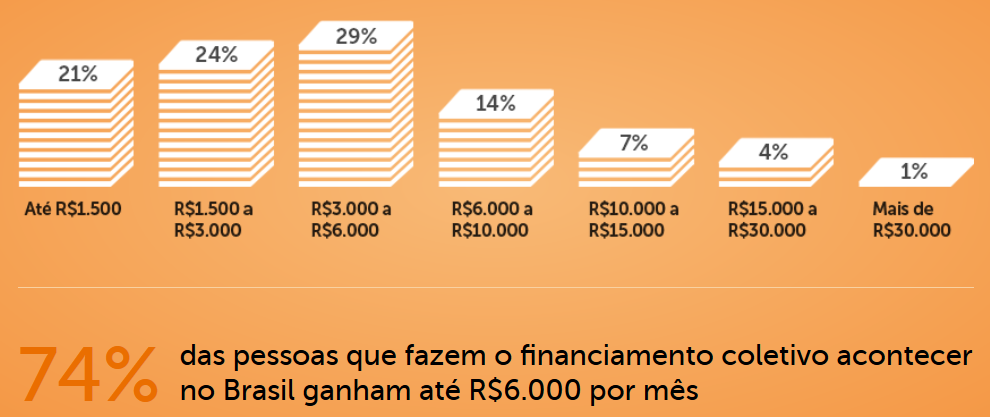
\includegraphics[scale=0.5]{fg1.png}
\caption{aixas de renda dos participantes do financiamento coletivo. \cite{CARTASECHORUS:2017}.}
\label{figura_1}
\end{figure}

\begin{figure}[!htb]
\centering
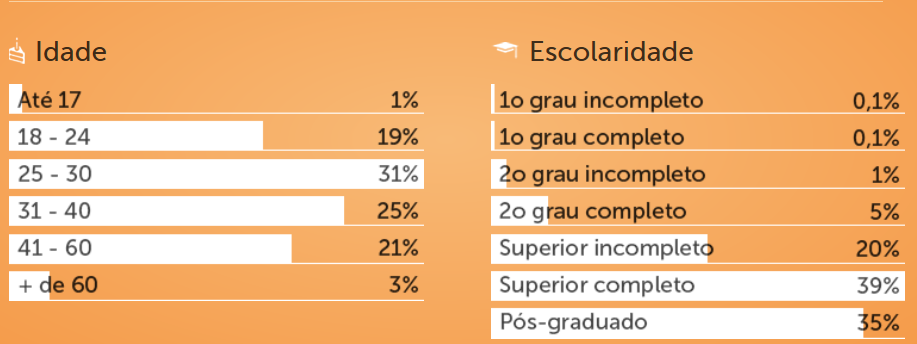
\includegraphics[scale=0.5]{fg2.png}
\caption{Faixa etária e nível de escolaridade dos participantes do financiamento coletivo\cite{CARTASECHORUS:2017}.}
\label{figura_2}
\end{figure}

Andrade \cite{ANDRADE:2017} descreve que atualmente, o \textit{Crowdfunding}  é praticado em mais de 160 países, segundo o relatório do \textit{The Crowdfunding  Centre}. Em 2014 foram arrecadados cerca 16,2 bilhões de dólares no mundo por meio do \textit{Crowdfunding} , um aumento de 167 \% em relação ao ano anterior, com uma arrecadação de 6 bilhões de dólares \cite{PASCOAL:2017}. No entanto, está fenômeno que se apresenta bastante difundido em outros países, como os Estados Unidos, ainda não possui grande expressividade no Brasil. Um exemplo disso, é o fato de apenas em 2015 o valor de arrecadações a nível mundial por meio do financiamento coletivo girar em torno de 9,4 bilhões de dólares, enquanto que no Brasil os 32 milhões de reais movimentados pelo \textit{Catarse} em seus quatro anos de funcionamento, representam apenas 0,1 \% desse total (\cite{ALVES:2017}.

Apesar disso, a população brasileira possui um forte caráter empreendedor, característica marcante principalmente em cenários como o atual com uma alta taxa de desemprego, onde o financiamento coletivo por ser menos burocrático e mais viável do que outras formas de financiamento, desponta como uma alternativa bastante interessante. Assim, espera-se que este tipo de pratica cresça no país nos próximos anos, como ocorreu e ocorre em outros países. Vale ressaltar que, campanhas com intuito social e/ou ambiental também possuem um forte apelo entre as campanhas nacionais.

%------------------------------------------------
% Seção 7
%------------------------------------------------
\section{Considerações Finais}

Como podemos compreender, através do que foi discutido no texto, o \textit{Crowdfunding}  possibilita o desenvolvimento de várias ideias que dificilmente conseguiriam alcançar o público com tanta clareza e rapidez. Essa “nova” abordagem do mercado de investimento proporcionou um grande aumento em projetos que antes não receberiam investimentos, através dos métodos tradicionais que é a apresentação do projeto para as empresas investirem nele. Como as empresas visam mais o seu lucro ou alguma forma de gerar marketing de seu produto para lucrarem, os projetos que elas investiriam seriam aqueles que suprissem suas necessidades. Assim, deixando de lado projetos com características culturais ou ambientais, que não traria retorno lucrativo, empobrecendo e desestimulando esse tipo de iniciativa.

Com a ideia de financiamento foi possível quebrar esse paradigma que impedia o investimento em projetos culturais. Com o público final podendo contribuir para ter acesso a projetos que os beneficiassem culturalmente. E não só os projetos culturais se beneficiaram com isso, através dessa nova forma de arrecadação de recursos abriu um novo mercado de empreendedores que possuem ideias de proporções pequenas, mas também de ideias que não pareceriam interessantes para as indústrias, mas que deram muito certo depois de alcançarem suas metas e desenvolverem seu produto. 

Além de uma maior facilidade de iniciar uma campanha na plataforma de financiamento coletivo, e sua forma de divulgação podendo ser através dá própria plataforma, as redes sociais também facilitam muito essa divulgação, atraindo cada vez mais pessoas e \textit{startup} com novas ideias para esse tipo de arrecadação de recursos.

%--------------------------------------------------------------------------------------------------
%--------------------------------------------------------------------------------------------------
% Define o arquivo BIB (bibliografia)
%--------------------------------------------------------------------------------------------------
%--------------------------------------------------------------------------------------------------
\bibliographystyle{bmc-mathphys}   % NAO EDITAR!
\bibliography{artigo_bibliografia} % NAO EDITAR! - Bibliography file (usually '*.bib' )

\vspace{1.0cm}

\begin{table}[h!]
\centering
\begin{tabular}{lp{8cm}}
 \raisebox{-\totalheight}{
\includegraphics[width=0.3\textwidth, height=50mm]{f1.png}} &  
  \vspace{0.1cm} Ricardo de Andrade Maia nasceu em Catolé do Rocha, interior do estado brasileiro Paraíba. Atualmente é
  graduando em Ciência da Computação pela Universidade Federal de Campina Grande (UFCG) e está
cursando o quarto semestre. Tem grande interesse em pesquisa na área de Desevolvimento Mobile e Desevolvimento de Games\\
  \raisebox{-\totalheight}{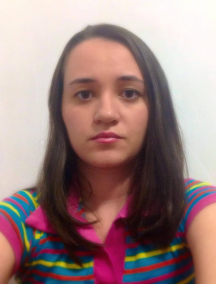
\includegraphics[width=0.3\textwidth, height=50mm]{f2.png}} &  
  \vspace{0.1cm} Danielle de Lima Vieira nasceu em Catolé do Rocha no estado da Paraíba. Atualmente é
  graduando em Ciência da Computação pela Universidade Federal de Campina Grande (UFCG) e está
cursando o quarto semestre. Tem grande interesse em pesquisa na área de Mobile e Desevolvimento, Desevolvimento de Games e computação grafica 3d. \\
  \raisebox{-\totalheight}{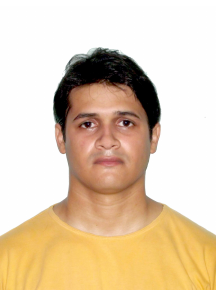
\includegraphics[width=0.3\textwidth, height=50mm]{f3.png}} &  
  \vspace{0.1cm} Damião Robson Domiciano 29 de Janeiro de 1988 em Santa Luzia, interior do estado brasileiro Paraíba. Atualmente é
  graduando em Ciência da Computação pela Universidade Federal de Campina Grande (UFCG) e está
cursando o terceiro semestre. Tem grande interesse em pesquisa na área de Análilse de Dados (AD).  \\
  \raisebox{-\totalheight}{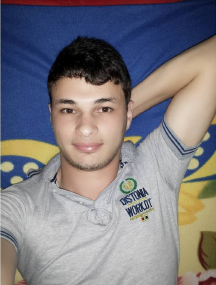
\includegraphics[width=0.3\textwidth, height=50mm]{f4.png}} &  
  \vspace{0.1cm} Lucas Venancio Duarte 14 de Novembro de 1996 em Alagoa Nova, interior do estado brasileiro Paraíba. Atualmente é
  graduando em Ciência da Computação pela Universidade Federal de Campina Grande (UFCG) e está
cursando o terceiro semestre. Tem grande interesse em pesquisa na área de Inteligência artificial (IA). \\

\end{tabular}
\end{table}

\begin{table}[h!]
\centering
\begin{tabular}{lp{8cm}}
\raisebox{-\totalheight}{
\includegraphics[width=0.3\textwidth, height=50mm]{f5.png}} &  
  \vspace{0.1cm} Adísio Pereira Fialho Júnior nascido no dia  22 de Janeiro de 1995 na cidade Cuité, interior do estado brasileiro Paraíba.
  Atualmente esta graduando em Ciência da Computação pela Universidade Federal de Campina Grande (UFCG) e está
  cursando o quarto semestre. Tem grande interesse em pesquisa na área de PERÍCIA COMPUTACIONAL.\\
\end{tabular}
\end{table}

%\end{tabular}
%\end{table}

%--------------------------------------------------------------------------------------------------
% FIM DO ARTIGO
%--------------------------------------------------------------------------------------------------
\end{document}
